%~~~~~~~~~~~~~~~~~~~~~~~~~~~~~~~~~~~~~~~~~~~~~~~~~
% {\jap riichi} Book 1, Chapter 1: Online
%~~~~~~~~~~~~~~~~~~~~~~~~~~~~~~~~~~~~~~~~~~~~~~~~~

\chapter{Introduction to {\jap tenhou} (天鳳)} \label{ch:tenhou}

\section{Why play online?}

Playing mahjong online is an excellent way to practice your mahjong skills. You don't need any mahjong equipment to play; you don't need to coordinate with your mahjong friends to find the time and place that work for the all four of you. You can simply open your computer and access one of many online mahjong platforms. As long as you have an internet connection, you can play mahjong any time, anywhere, and for any length of time. 

\bigskip
Another advantage of online playing is that you can easily keep the record of your playing history and obtain detailed statistics from all the games you play. Analyzing these statistics will help you identify what skill sets you need to work on. You can also show your game record to your friends and ask for their opinions about particular choices you've made in a game. 

\begin{wrapfigure}{r}{50mm}
\vspace{-20pt}
\begin{center}
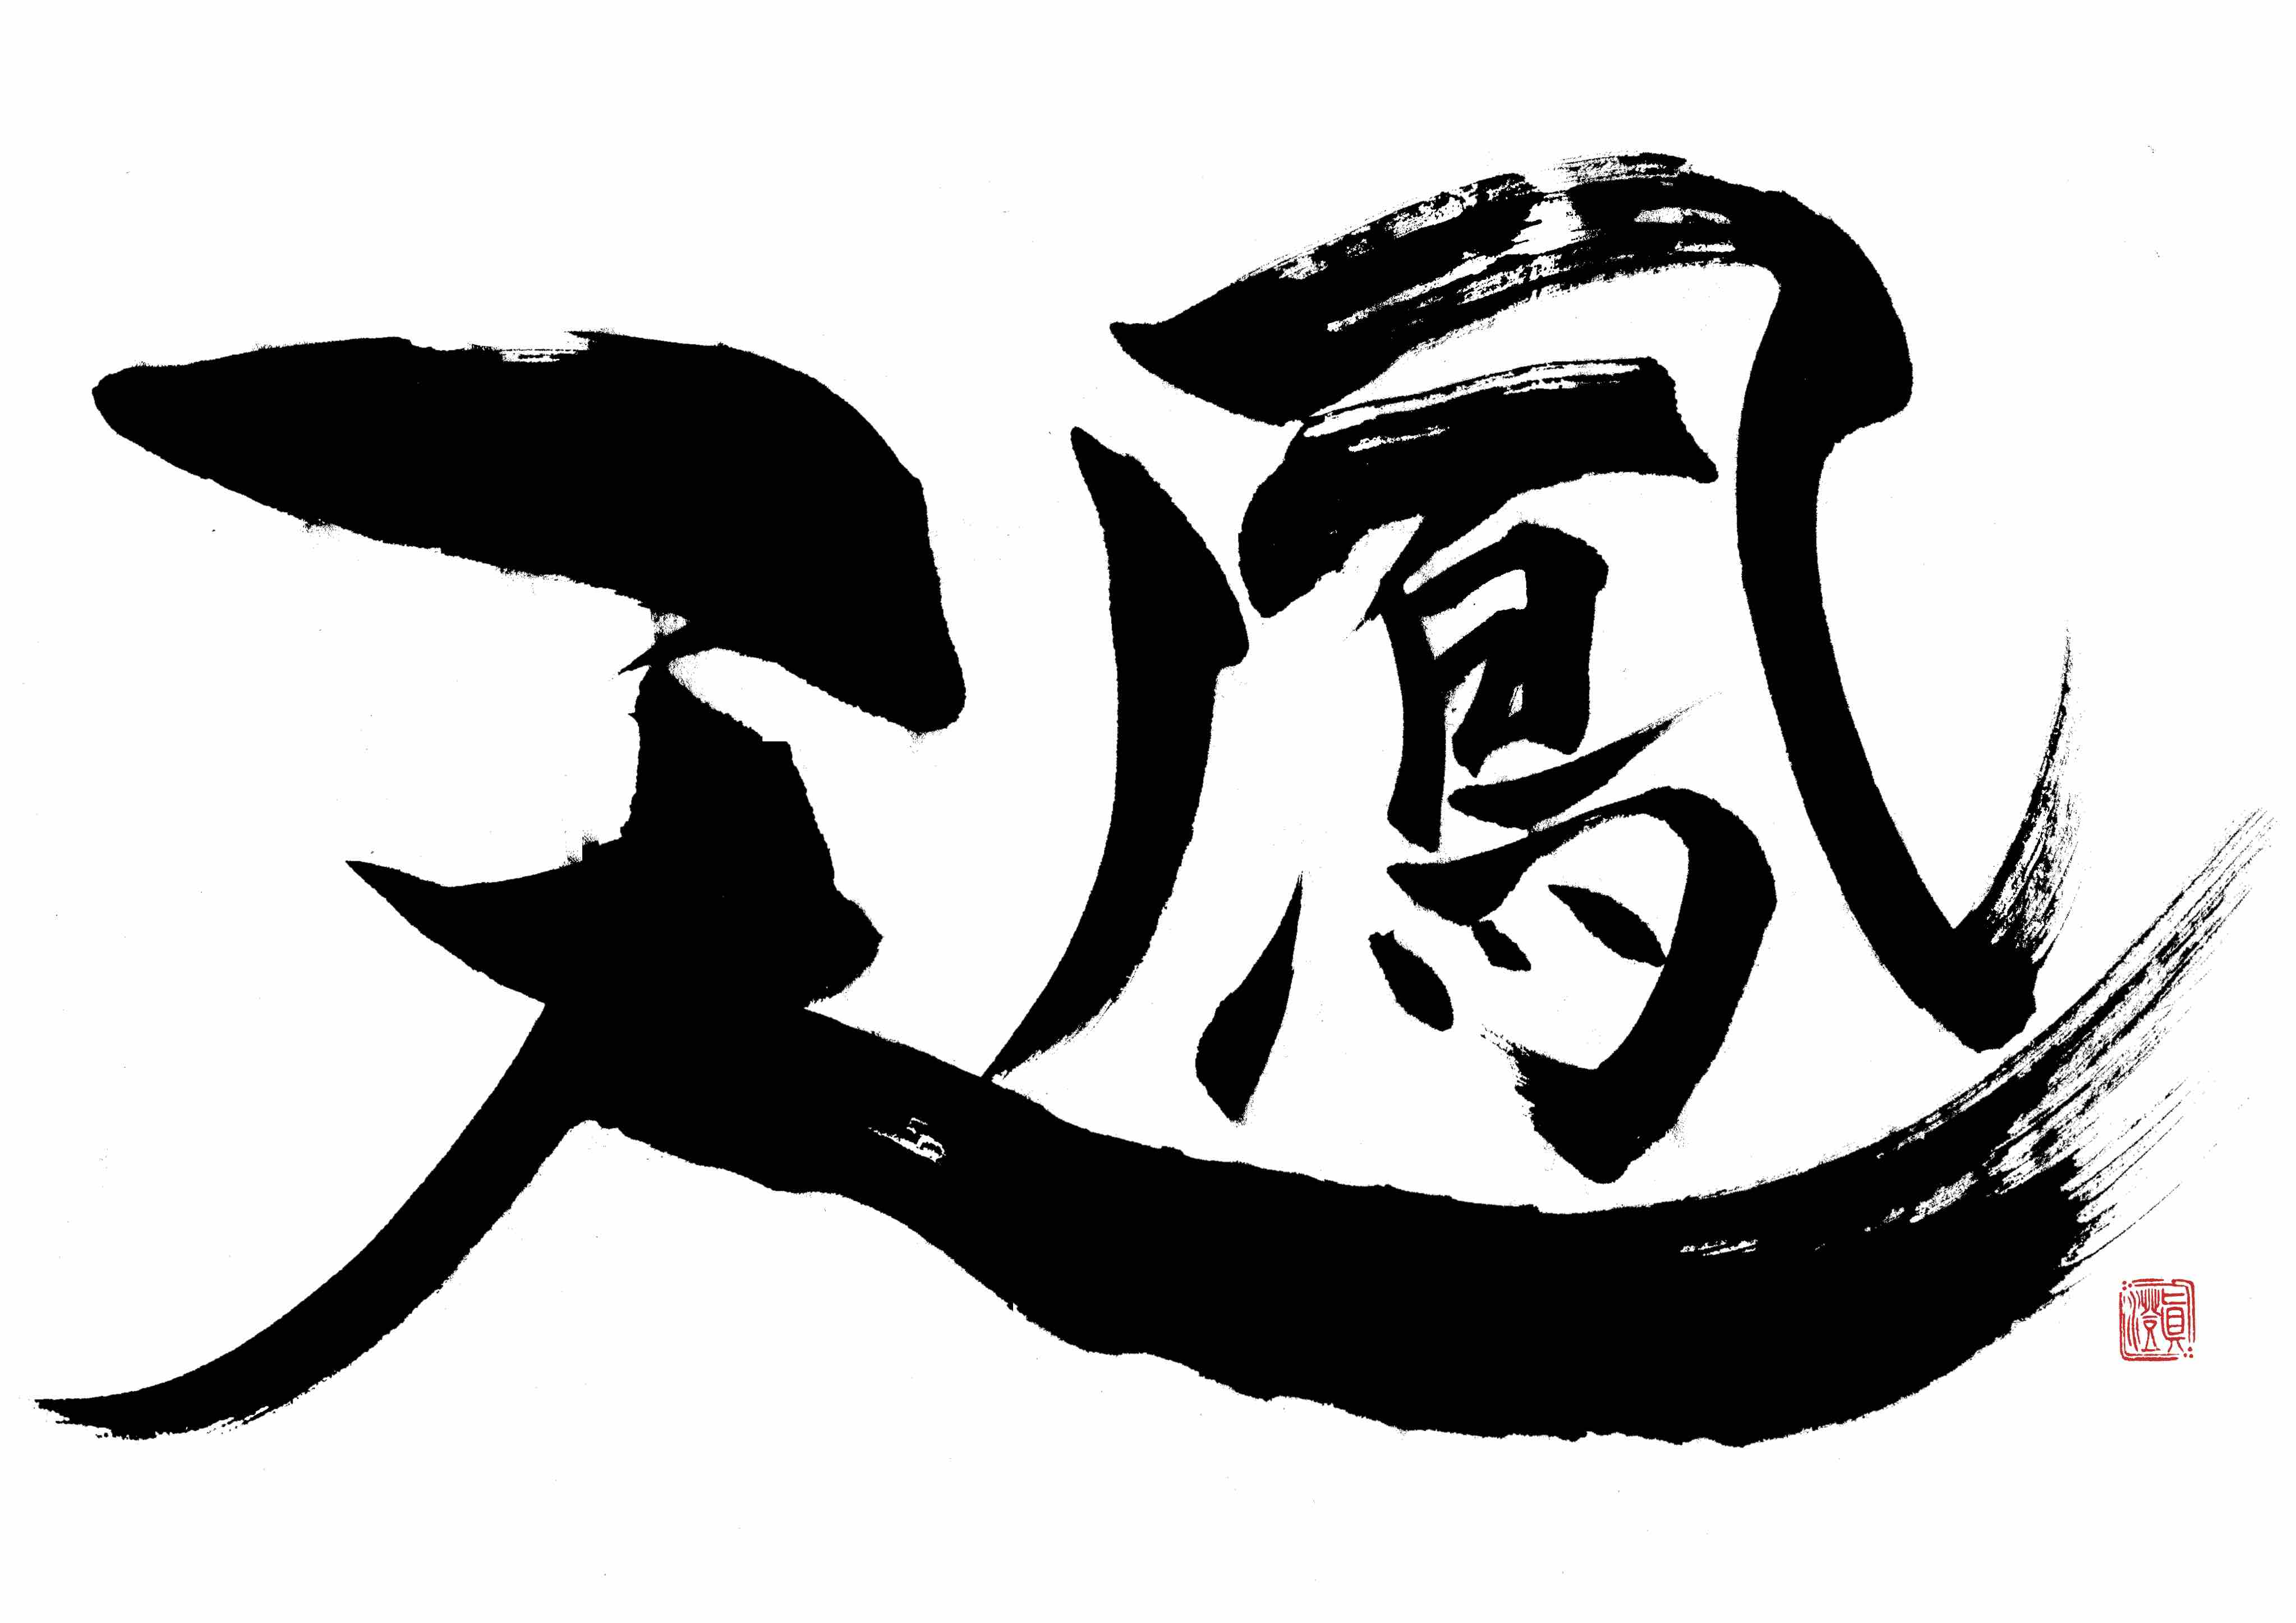
\includegraphics[width=.43\textwidth,clip]{figs/tenhou_logo_raw_wb}
\end{center}
\vspace{-20pt}
\end{wrapfigure}

\bigskip

天鳳 ({\jap tenhou}) is arguably the most popular online mahjong platform in the world. As of December, 2015, there are over three hundred thousands active players on {\jap tenhou}.\footnote{To be exact, it has 304,534 active players and 3,566,353 registered players as of 20 December, 2015.} A lot of professional mahjong players from Japan now play {\jap tenhou}. There are also some {\jap tenhou} players who have later become professional after practicing their skills on {\jap tenhou}. It has become a common understanding among players in Japan that your rank and rating at {\jap tenhou} are one of the most reliable indicators of your mahjong skill levels. 
To get you started, this chapter explains how to set up an account at {\jap tenhou} and provides some basic operation manual. 

\section{Setting up an account}
One of the challenges for European players in setting up an account at {\jap tenhou} would be that almost everything is written in Japanese. However, you will only need a minimal level of Japanese to get by, and this chapter will walk you through the process. 

%\newpage
\bigskip

\noindent First, go to the {\jap tenhou} webpage (\url{http://tenhou.net/}). 

\begin{center}
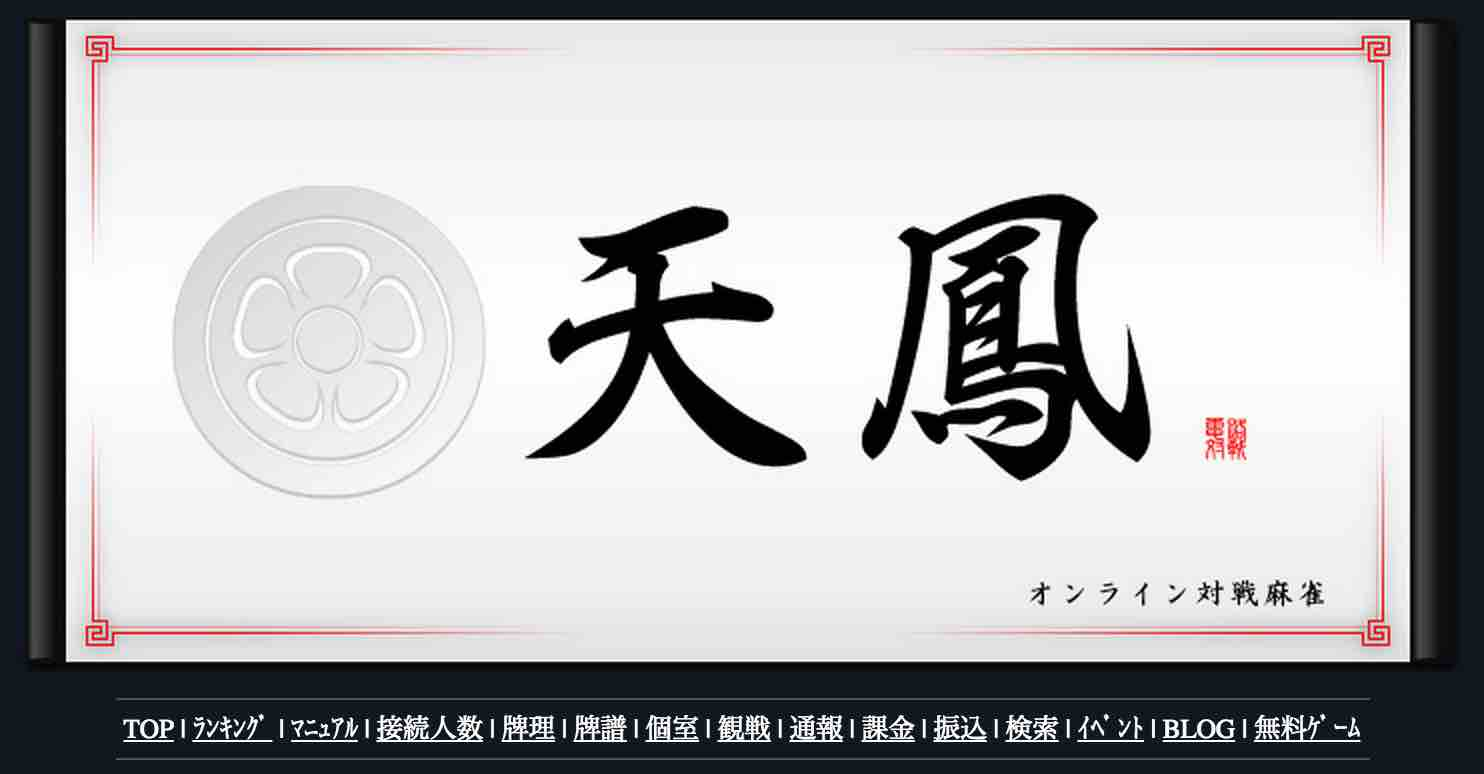
\includegraphics[width=.7\textwidth,clip]{figs/tenhou0.jpg}
\end{center}

%\bigskip

\noindent Scroll down and click either the PLAY button (to play in a pop-up window) or a link just below the button (to play in the current window) that reads \underline{このウィンドウで開く}.

\vspace{40pt}

%\begin{center}
\begin{overpic}[width=.7\textwidth,clip]{figs/tenhou1.jpg}
\linethickness{3pt}
\put(260,65){\color{MyRed} \vector(-2,-1){35}}
\put(230,78){\color{MyRed}\small Click here to play}
\put(265,65){\color{MyRed}\small in a pop-up}
\put(265,50){\color{MyRed}\small window.}
\put(260,18){\color{MyRed} \vector(-1,0){35}}
\put(240,27){\color{MyRed}\small Click this link to}
\put(265,13){\color{MyRed}\small play in the}
\put(240,0){\color{MyRed}\small current window.}
\end{overpic}
%\end{center}

\bigskip
%\newpage

Then, on the next page (either in a pop-up window or in the current window), you'll see something like the following: 

\begin{center}
\begin{overpic}[width=.8\textwidth,clip]{figs/tenhou3.jpg}
\linethickness{1pt}
\put(120,-5){\color{MyRed} \vector(0,1){17}}
\put(170,-5){\color{MyRed} \vector(0,1){17}}
\put(60,-13){\color{MyRed} Flash version}
\put(160,-13){\color{MyRed} Web version}
\end{overpic}
\end{center}

\bigskip

The bottom line will initially read LOADING... / 再読み込み, but in a few seconds it will change into >>Flash版サーバに接続 | Web版$\beta$サーバに接続. Then, click on the Flashサーバに接続 link if you are accessing from a flash-capable device such as your PC; alternatively, click on the Web版$\beta$サーバに接続 link if you are accessing from a smart phone or tablet. 
If it doesn't change into >>Flash版サーバに接続 | Web版$\beta$サーバに接続 within 10 seconds or so, you may want to click on the 再読み込み link right next to LOADING, which will prompt the browser to reload the page. 
Clicking on either of the Flash/Webサーバに接続 links will take you to the log-in entrance of {\jap tenhou}. Explanations below are based on the Flash version. 

\bigskip

\begin{center}
\begin{overpic}[width=.8\textwidth,clip]{figs/tenhou4.jpg}
\linethickness{2pt}
\put(70,-10){\color{MyRed}\vector(0,1){30}}
\put(10,-20){\color{MyRed} \small Registration}
\put(120,-10){\color{MyRed} \vector(0,1){30}}
\put(90,-20){\color{MyRed} \small ID field (likely to be blank at first)}
\end{overpic}
\end{center}

%\vspace{10pt}

\bigskip
When you first visit this page, the ID field right next to the 新規ID登録 button is likely to be blank, as shown in the picture above. This is because you haven't registered an account. 
In order to create an account, click on the 新規ID登録 (New ID Registration) button on the left. 

\begin{center}
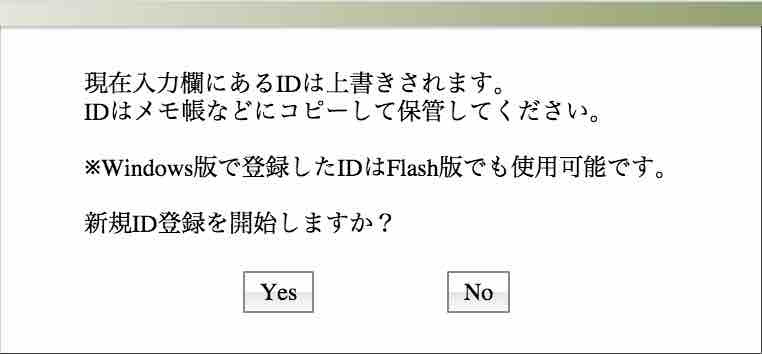
\includegraphics[width=.6\textwidth,clip]{figs/tenhou5.jpg}
\end{center}

A pop-up message will show up, warning you that whatever ID that is currently shown in the ID field (if any) will be overwritten with a new ID and that you may want to copy and paste the current ID (if any) into some text file or similar. Do so if you do see an old ID in the ID field, just to be safe. If the ID field is blank, just click the Yes button, which will open yet another pop-up message. 

\begin{center}
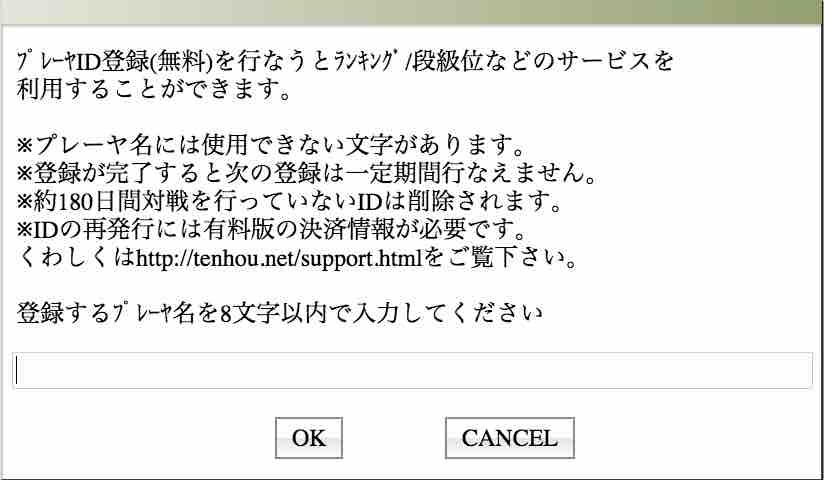
\includegraphics[width=.6\textwidth,clip]{figs/tenhou6.jpg}
\end{center}

\noindent It is telling you the following:
\bi \itemsep0.1em
\i You can create a player ID for free, and doing so is necessary if you want to earn a rank ({\jap kyu / dan}) and rating. 
\i Some characters or character combinations are not allowed in player names.
\i Once you register, you cannot register another account for a given period (7 days).
\i If you don't play for 180 days, your ID may be deleted.
\i A player name must have 1-8 characters.
\ei

Type in a player name you'd like to have (8 characters or less) into the blank field at the bottom and click OK. 
You cannot change your player name later, so choose wisely. If the player name you type in is already taken by another player, it gives you an error message, as follows:

%\begin{wrapfigure}{r}{60mm}
\begin{center}
\begin{overpic}[width=.5\textwidth,clip]{figs/tenhou8.jpg}
\put(10,0){\color{MyRed} This player name is taken.}
\end{overpic}
\end{center}
%\vspace{-10pt}
%\end{wrapfigure}

Click OK, and type in another name. If successful, you'll see a new message asking you to confirm that you want to register an account with the player name provided. 

\begin{center}
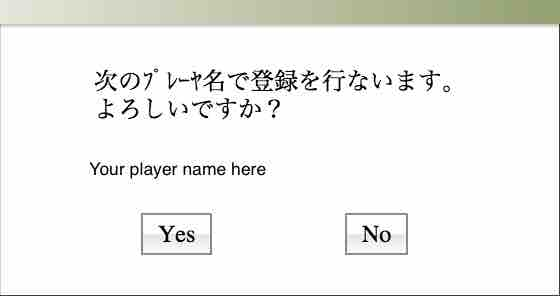
\includegraphics[width=.55\textwidth,clip]{figs/tenhou9.jpg}
\end{center}

%\bigskip

\noindent Click Yes and you'll see another message as follows:
\begin{center}
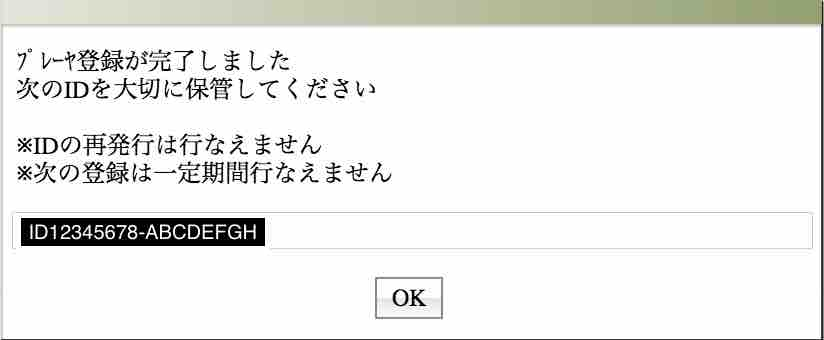
\includegraphics[width=.8\textwidth,clip]{figs/tenhou10.jpg}
\end{center}

The 19-digit alpha-numeric code that starts with ``ID'' (shown in white on a black background) is your unique player ID (it is ID12345678-ABCDEFGH in the picture above). I suggest you save your ID in a text file or something so that you don't lose it. They cannot re-issue your player ID (unless you have a paid membership and hold a rank higher than 七段). 

\bigskip

Clicking OK will take you back to the log-in entrance page, but this time you should see your player ID in the ID field.

%\bigskip
\begin{center}
\begin{overpic}[width=.8\textwidth,clip]{figs/tenhou11.jpg}
\linethickness{2pt}
\put(80,-10){\color{MyRed}\vector(1,1){37}}
\put(10,-20){\color{MyRed}\small Your player ID}
\put(175,-10){\color{MyRed}\vector(0,1){37}}
\put(100,-22){\color{MyRed}\small Choose 男 (male voice) or 女 (female voice)}
\put(220,70){\color{MyRed}\vector(-1,-2){20}}
\put(205,115){\color{MyRed}\small Can choose}
\put(205,98){\color{MyRed}\small プレミアム or}
\put(205,80){\color{MyRed}\small エコノミー.}
\end{overpic}
\vspace{10pt}
\end{center}

\bigskip
You can make several choices before entering the main page. First, you can choose male or female voice (for {\jap pon} / {\jap chii} / {\jap riichi}, etc.) by clicking on the button right next to the ID field. You can choose a different gender each time you log in to the main lobby. Second, you can choose プレミアム (premium) or エコノミー (economy) version. The premium version has better graphics, so I suggest you choose the premium version. 

\bigskip
If you are happy with your choices, you can enter the main page by clicking on the OK button on the right. 

\newpage

\section{The main page}

Here is what the {\jap tenhou} main page looks like when you first log on in. 
The right half of the main page shows your statistics (currently all the fields are blank because you haven't played any games), and the left half shows the games you can play and some other features. 

\bigskip

\begin{center}
\begin{overpic}[width=.8\textwidth,clip]{figs/tenhou_lobby.jpg}
\linethickness{2pt}
\put(20,-15){\color{MyRed}\small Menu}
\put(70,-15){\color{MyRed}\small Cancel (to cancel a reservation)}
\put(50,-5){\color{MyRed}\vector(0,1){20}}
\put(110,-5){\color{MyRed}\vector(0,1){20}}
\put(-45,150){\color{MyRed}\small Main tabs}
\put(-40,130){\color{MyRed}\small Sub tabs}
\end{overpic}
\end{center}

\bigskip

In the second line of the left hand side, you see three numbers. In the example above, they are 1857, 915, and 118 (the numbers will be different on your screen). These numbers show that 1857 players are currently online, 915 players are waiting, and 118 players are about to finish their games. 

\bigskip
Below these three numbers, there are six main tabs, which read 段位戦, 雀荘$\beta$, 技能$\beta$, 観戦, 牌譜, and ヘルプ. The 段位戦 tab is the main lobby where we play games (段位戦 reads {\jap dan i sen} in Japanese; it means ranking matches). Under the 段位戦 tab, there are four sub-tabs, which read 一般, 上級, 特上, and 鳳凰, corresponding to four different rooms. At first you can only play at tables in the 一般 room. 
Let's first go to the 段位戦 tab, and choose the 一般 sub-tab. 

\subsection*{Making reservations}
In each of the four rooms (i.e., 一般, 上級, 特上, and 鳳凰), there are 12 different variants of Riichi Mahjong games you can choose from. 

\bigskip

Games in the left column (under 東風戦 {\jap tonpusen}) are East-only games (there is no South rounds in these games),\footnote{In a special circumstance where no player gets 30000 or more points by the end of East-4, the game continues into the South round.} and games in the right column (under 東南戦 {\jap tonnansen}) are more standard East-South games that have both East and South rounds.\footnote{Just like East-only games, when there is no player who has 30000 or more points by the end of South-4, the game continues into the West round. 
}

\begin{center}
\begin{overpic}[width=.6\textwidth,clip]{figs/ippan.jpg}
\linethickness{2pt}
\put(-68,120){\color{MyRed}\small Closed {\jap tanyao}}
\put(-64,100){\color{MyRed}\small Open {\jap tanyao}}
\put(-67,78){\color{MyRed}\small With red fives}
\put(-23,57){\color{MyRed}\small Fast}
\put(-60,33){\color{MyRed}\small Three-player}
\put(-40,13){\color{MyRed}\small Fast (3p)}
\put(67,-10){\color{MyRed}\small East-only}
\put(135,-10){\color{MyRed}\small East--South}
%\put(220,120){\color{MyRed}\vector(-1,0){20}}
\put(200,120){\color{MyRed}\small 1 player waiting}
\put(200,105){\color{MyRed}\small 44 players playing}
\end{overpic}
\end{center}


\bigskip
Games in the first row (喰断ナシ {\jap kuitan nashi}) are unusual games where open {\jap tanyao} (All Simples) is not allowed; you have to have a concealed hand to claim {\jap tanyao}.\footnote{{\jap kuitan} means ``open {\jap tanyao}'' and {\jap kuitan nashi} means ``without {\jap kuitan}'' in Japanese.} There is no red five in these games, either. 
Open {\jap tanyao} is allowed in all the other games. Games in the second row are more standard games with open {\jap tanyao}, but they do not have red fives. 
Games in the third row have three red fives. This is arguably the most standard type of {\jap riichi} mahjong game played in Japan as of now. 
Games in the fourth row have the same rule as those in the third, but the time limit on each action is more strict. 
Games in the fifth and sixth rows are three-player games, where open {\jap tanyao} and red fives are both allowed. 

\bigskip
The set of numbers delimited by a colon in each cell represent the numbers of players currently waiting and playing the game, respectively. For example, the first row in the left column shows 3:24, which means that 3 players are waiting in queue after signing up for a game, and 24 players are currently playing East-only, closed {\jap tanyao} games. As it happens, East-South games with red fives are usually the most popular on {\jap tenhou}, followed by East-only, fast games. 

\bigskip
To sign up for a game, click on the \fbox{予約} (reservation) button in the corresponding cell. You can make as many reservations as you want; you will be given a seat at a table that first becomes available. If you make multiple reservations, other reservations will be automatically canceled when you start playing at another table. To cancel all the reservations at once, click on the \fbox{キャンセル} (Cancel) button at the bottom right of the left-hand side of the main page. The cancel button becomes active (clickable) only after you make a reservation. 

\section{Playing a game}

\begin{wrapfigure}{r}{50mm}
\vspace{-20pt}
\begin{center}
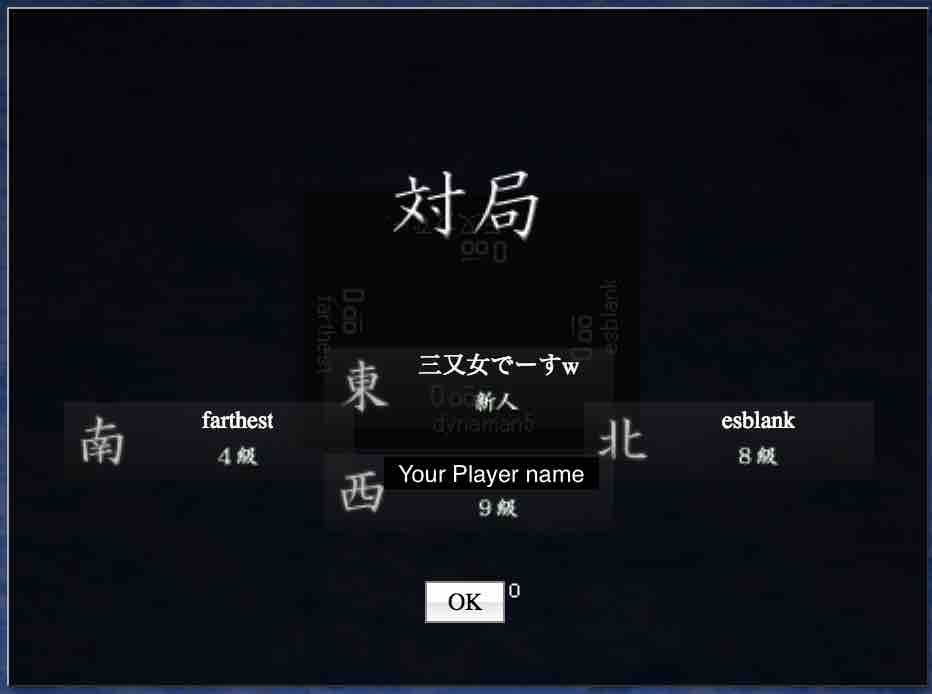
\includegraphics[width=.4\textwidth,clip]{figs/taikyoku}
\end{center}
\vspace{-20pt}
\end{wrapfigure}

Once a slot becomes available for you, you will be taken to a game table along with three other players. A black pop-up screen (see right) will appear. The game will start in 10 seconds (if all the four players click on the OK button, the game will start immediately). Each player is randomly assigned to East, West, South, or North. In the example below, my initial seat wind is North (北). 

The {\jap tenhou} interface is quite intuitive so you won't need much instruction. 
Once a hand begins, tiles are dealt automatically. You also automatically draw a tile when your turn comes. 
In each turn, click on the tile you want to discard. 

%\begin{wrapfigure}{r}{60mm}
\begin{center}
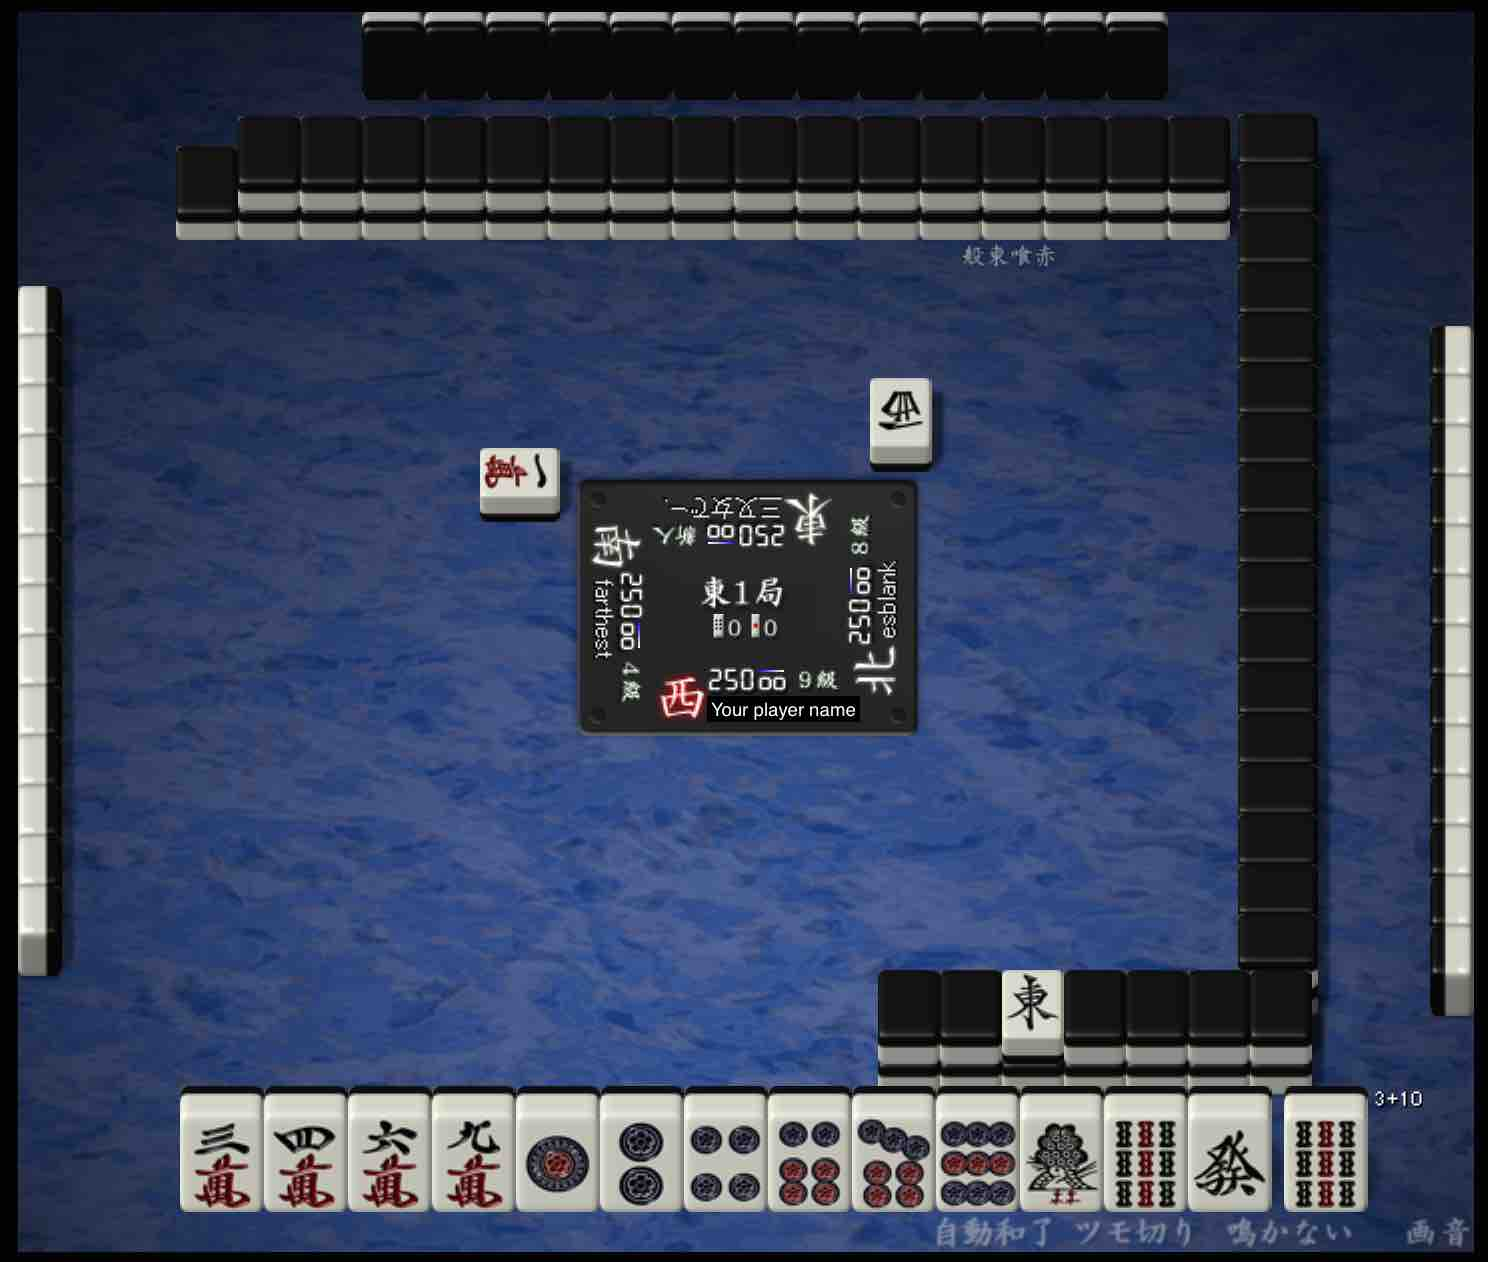
\includegraphics[width=.6\textwidth,clip]{figs/interface.jpg}
\end{center}
\vspace{-25pt}
%\end{wrapfigure}

\bigskip
Each action is timed. At a standard (non fast) table, you have 5 seconds to discard a tile. In addition, you are given a total allowance of 10 seconds in each hand. That is, even when you use up the 5 seconds allocated to you in a particular turn, you will be given the maximum of additional 10 seconds (minus the seconds you have already used up in previous turns in the hand). For example, when you use 5 + 4 seconds in the first turn, the remaining allowance reduces to $10 - 4$ = 6 seconds in this hand. Therefore, the next time you use up the first 5 seconds, you will be given only 6 more seconds. The allowance will increase by 1 second (up to 10 seconds) each time you make your discard choice in less than 1 second. The allowance will revert to 10 seconds when the next hand begins. At fast tables, each action must be done in 3 seconds, with a total allowance of 5 seconds.

\subsection{Calling / melding}
When a call becomes available, a box with a call name will show up to prompt your reaction. 
The call prompts are written in Japanese. The good news is that they are relatively simple and easy to guess from the context. It would be enough to memorize the following eight mahjong words in Japanese. 

\subsubsection{1. リーチ {\jap riichi} \textipa{[r\'\textsci\textlengthmark t\textesh]}} 
You can call {\jap riichi} when you have (1) a closed ready hand, (2) at least 1000 points left, and (3) at least one turn left to draw. When all of the three conditions are met, a translucent box that reads リーチ in white letters will pop up in your turn. 
\begin{center}
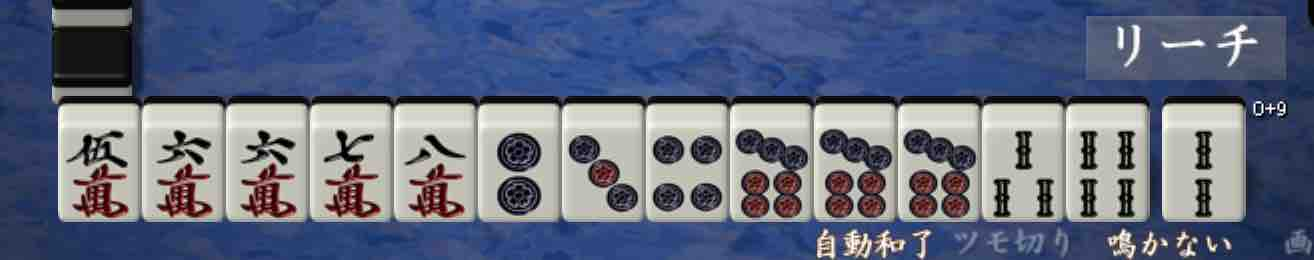
\includegraphics[width=.7\textwidth,clip]{figs/riichi.jpg}
\end{center}
If you want to {\jap riichi}, you \underline{must click on the リーチ box first}, then click on the tile you want to discard. Once you click on the リーチ box, you cannot call it off. Clicking on the リーチ box also makes it impossible to discard a tile that does not make the hand ready. In the above example, tiles other than {\large \wan{5}\wan{6}\wan{8}\tong{7}} will become unclickable once you click on the リーチ box. If you do not want to call {\jap riichi}, just click on the tile you want to discard. 

\subsubsection{2. ロン {\jap ron} \textipa{[r\'\textopeno\ng]}}
A ロン box will pop up whenever you can legitimately declare {\jap ron} on an opponent's discard or intercept a melded Kong. In other words, {\jap chombo} is made impossible on {\jap tenhou}. For example, when you are {\jap furiten}, a ロン box will not pop up because you cannot legally {\jap ron} with a {\jap furiten} hand. Whenever your hand is in a {\jap furiten} status, it is indicated with a フリテン ({\jap furiten}) sign in small translucent letters below your hand that looks like: 
\includegraphics[width=.12\textwidth,clip]{figs/furiten.jpg}.
If you don't click on the ロン box in time (i.e., in 5 or 3 seconds + allowance), it is assumed that you pass. 

\subsubsection{3. パス Pass (do nothing)}
Whenever a ロン box pops up, another box that reads パス (pass) will always accompany it. 
\begin{center}
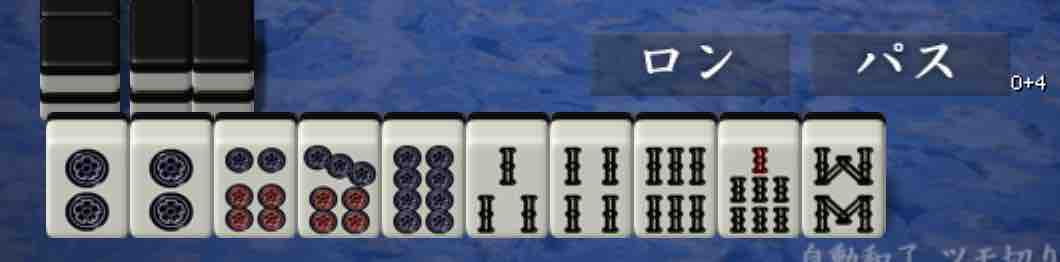
\includegraphics[width=.7\textwidth,clip]{figs/ron.jpg}
\end{center}
Click on the パス box immediately if you don't want to declare {\jap ron} on a discard. You would not want to pause for too long because that can look suspicious. A パス box will also pop up when other calling actions become available. 

\subsubsection{4. ツモ {\jap tsumo} \textipa{[ts\'umo]}}
A ツモ box will pop up when you can legitimately declare {\jap tsumo} with your draw. 

\subsubsection{5. ポン {\jap pon} \textipa{[p\'\textopeno\ng]}}
When calling {\jap pon} becomes available, a ポン box will pop up right above the tiles in your hand with which to call {\jap pon}. A パス box will also pop up. If you want to call {\jap pon}, mouseover the tiles in your hand with which to call {\jap pon}. Then the candidate tiles will stick out, as follows:
\begin{center}
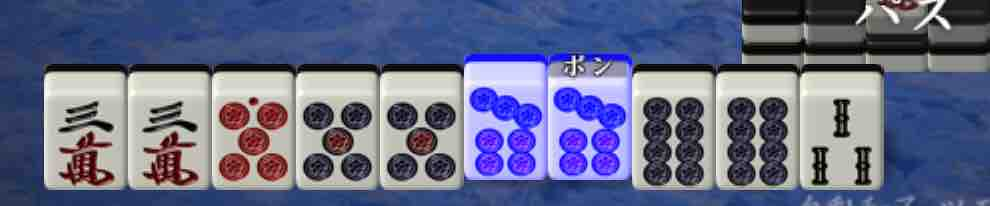
\includegraphics[width=.7\textwidth,clip]{figs/pung.jpg}
\end{center}
Click on them to call {\jap pon}. If you click on the パス box or don't do anything in time, it is assumed that you pass. 

\subsubsection{6. チー {\jap chii} \textipa{[t\textesh\'\textsci\textlengthmark]}}
{\jap Chii} calls are done in a similar way. When it becomes available, a small sign that reads チー will pop up right above the tiles in your hand with which to call {\jap chii}. 

\begin{center}
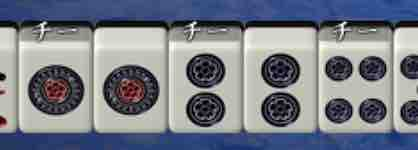
\includegraphics[width=.4\textwidth,clip]{figs/callchii_alt.jpg}
\end{center}

When you have multiple sets of tiles with which to {\jap chii}, as is the case in the above picture, mouseover the candidate tiles to choose. In the picture above, the left player discarded a {\large \tong{3}} and you can {\jap chii} it with either {\large \tong{1}\tong{2}} or {\large \tong{2}\tong{4}}. If you want to {\jap chii} it with {\large \tong{1}\tong{2}}, mouseover the {\large\tong{1}} then the {\large \tong{1}} and a {\large \tong{2}} will stick out so you can click on them. If you want to {\jap chii} it with {\large \tong{2}\tong{4}}, mouseover the {\large\tong{4}} then a {\large \tong{2}} and the {\large \tong{4}} will stick out so you can click on them.

\subsubsection{7. カン {\jap kan} \textipa{[k\'\textturnv\ng]}}
Calling {\jap kan} on a discard is similar to calling {\jap pon}. To build a melded {\jap kan} by extending a melded {\jap pon}, you need to mouseover the melded {\jap pon} until a small sign that reads カン appears below the {\jap pon}. To call a concealed {\jap kan}, mouseover the four tiles you want to {\jap kan} then the tiles will stick out, accompanied by a small sign that reads カン below them. Click on them to call {\jap kan}. 

\subsubsection{8. 九種九牌 {\jap Kyushu Kyuhai}}
When you have nine different terminals and honors after the first draw in an uninterrupted first set of turns, you can declare an abortive draw. When this becomes available, a box that reads 九種九牌 will pop up. Click on it if you want to declare an abortive draw. If you wish to continue with the hand, just click on the tile you want to discard. 

\subsubsection{Multiple boxes}

Sometimes you have multiple choices as to what to do with a given discard of your opponent. 
In the following example, you have a ready hand waiting for {\large \wan{2}-\wan{5}}, and the left player discarded a {\large \wan{5}}. You will be given the following three choices: 

\begin{center}
\begin{overpic}[width=.6\textwidth,clip]{figs/ron_pass.jpg}
\linethickness{2pt}
\put(100,70){\color{MyRed}\large {\jap Ron}}
\put(160,70){\color{MyRed}\large Pass}
\put(-45,34){\color{MyRed}\large {\jap Chii}}
\end{overpic}
\end{center}

\bi\itemsep.1em
\i Call {\jap ron}
\i Call {\jap chii}
\i Pass (do nothing)
\ei
To call {\jap ron} on the discarded {\large \wan{5}}, click on the ロン ({\jap ron}) box that pops up above your hand. If you want to do nothing, click on the パス (pass) box right next to the ロン box. Alternatively, if you want to call {\jap chii}, mouseover the two tiles you want to {\jap chii} with (in this case {\large \wan{3}\wan{4}}) and click on them. 


\subsection{Buttons}

The buttons at the bottom right corner allow you to toggle on/off some calling-related features. Each feature is turned off at the beginning of a new hand. 

\bigskip

\begin{center}
\begin{overpic}[width=.8\textwidth,clip]{figs/choices.jpg}
\put(-10,-13){\color{MyRed}\small Auto-call win}
\put(50,25){\color{MyRed}\small Auto discard draw}
\put(170,-13){\color{MyRed}\small No call}
\put(230,-13){\color{MyRed}\small Picture (画)}
\put(240,25){\color{MyRed}\small Sound (音)}
\end{overpic}
\end{center}

\bigskip

\subsubsection{自動和了 (Auto-call win)} 
If you turn this on, you will automatically win a hand when possible without clicking on ロン or ツモ boxes. In other words, the option of passing is unavailable when this is turned on. Keep in mind that this can be problematic at times when you intend not to win your hand from a particular opponent or on a particular tile. When this is turned on, the word 自動和了 is shown in white; when it is turned off, it is translucent. In the picture above, it is turned on. 

\subsubsection{ツモ切り (Auto discard draw)} 
If you turn this on, you will automatically discard whatever tile you draw. Turn this on when you have to go to toilet or somewhere but don't want to quit the game entirely. When you {\jap riichi}, this feature is automatically (and implicitly) turned on. In the picture above, it is turned off. 

\subsubsection{鳴かない (No call)}
If you turn this on, you will not be prompted to call {\jap chii}, {\jap pon}, or {\jap kan}. This feature is useful for hiding information about your hand's tile composition from your opponents. If you pause every time someone discards a certain tile you can call, your opponents might be able to guess what pairs of tiles you have and don't have. Drawing a deduction from such time lags constitutes an important skill in {\jap tenhou}. However, in order not to disadvantage players waiting to call {\jap chii} / {\jap pon} too much, time lags will also occur randomly (i.e., even when no one can call {\jap pon} / {\jap chii} on the discarded tile). 

\subsubsection{画 (Picture) and 音 (Sound effect)}
You can change the appearance of the tiles and/or mat or resize the window with the Picture button. You can turn on/off the sound effect (for {\jap riichi}, {\jap chii}, {\jap pon}, etc.) with the Sound button.

\subsection{Scoring}
When a player wins a hand, the score will be calculated automatically. A scoring board will pop up that shows the hand, {\jap dora} (and {\jap ura dora} if {\jap riichi} was declared), {\jap yaku} names and the associated number of {\jap fan}, minipoints, and the total hand value. 

\begin{center}
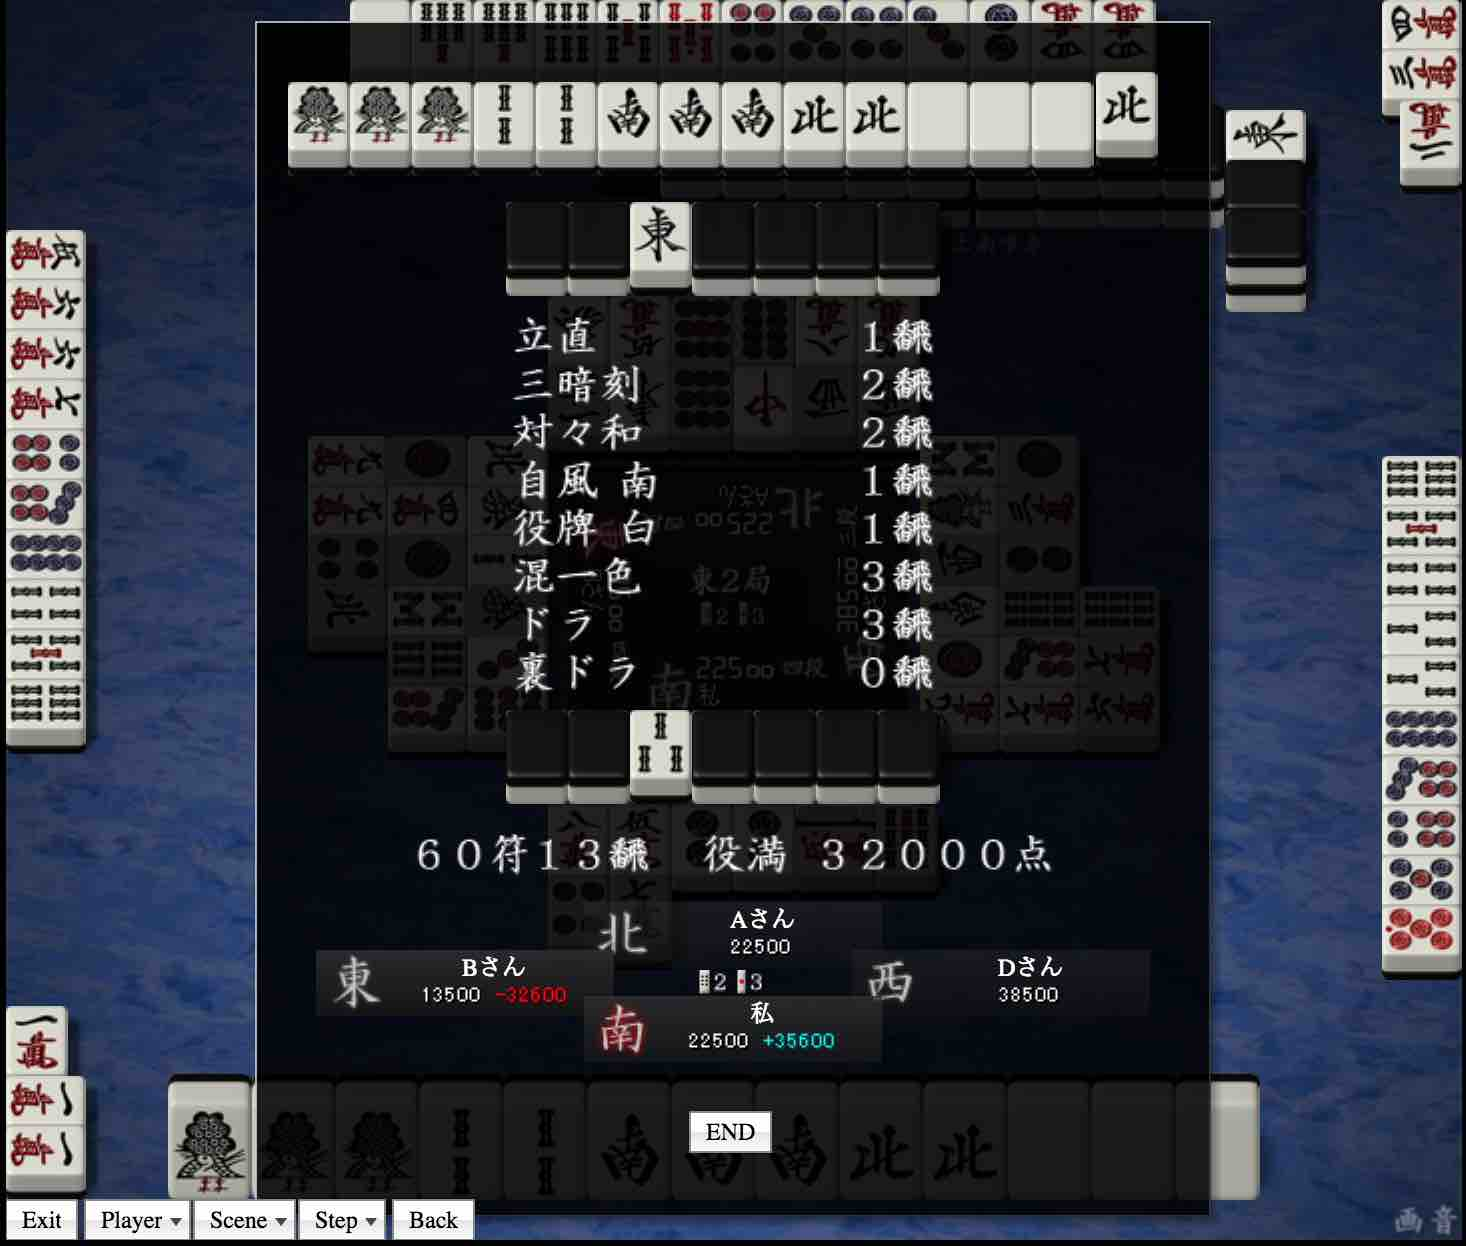
\includegraphics[width=.6\textwidth,clip]{figs/yakuman.jpg}
\end{center}
In the example above, the left player dealt into my hand that is worth 60 符 (minipoints) 13 飜 ({\jap fan}) = 32000 点 (points). {\jap Yaku} names will be shown in Japanese along with {\jap fan} counts. 
Table \ref{tbl:yakulist} at the end of this chapter lists all the {\jap yaku} names {\jap tenhou} recognizes. 


\subsection{Indicators}\label{sec:indicator}
The black rectangular board in the middle of the screen provides information about the proceeding of the game. 

\begin{center}
\begin{overpic}[width=.4\textwidth,clip]{figs/proceeding1}
\linethickness{2pt}
\put(150,82){\color{White} \vector(-2,-1){70}}
\put(-15,82){\color{White} \vector(2,-1){70}}
\put(150,80){\color{MyRed}\bf Number of}
\put(150,65){\color{MyRed}\bf {\jap riichi} bets}
\put(-60,73){\color{MyRed}\bf Counter}
%\begin{overpic}[width=.4\textwidth,clip,grid]{figs/proceeding2.jpg}
\end{overpic}
\end{center}
We can see that this is South-4, there is 0 counter and 0 {\jap riichi} bet, and it is the North player's turn. 
The West player is leading (44000 points), followed by the East player (26800), the North player (17400), and the South player (11800). Player's rank ({\jap kyu / dan}) is shown right next to their points. 

%\begin{wrapfigure}{r}{60mm}
\begin{center}
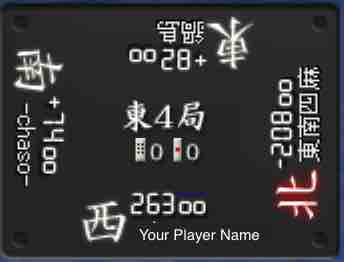
\includegraphics[width=.4\textwidth,clip]{figs/proceeding2}
\end{center}
%\vspace{-10pt}
%\end{wrapfigure}

\bigskip
If you mouseover the middle board, you will see the current point differences between you and each of your opponents. 
In the present example, the West player has $44000 - 26800 = + 17200$ more points than I do. If you are leading against another player, the point difference will be negative. For example, the South player has $11800$ so the point difference is $11800 - 26800 = -15000$. 

\bigskip
It is important to pay a close attention to these point differences, especially in the South round or when one of your opponents is at the risk of bankruptcy. In the current example, if someone wins a 6400 hand from the North player, he will go bankrupt and the game is terminated. Notice that West is currently ranked third, having 7200 less points than South and 8200 less points than East. In this case, winning a 6400 from North is not ideal for West because West will still be ranked third and the game is over, which is not the worst outcome but far from ideal.\footnote{As we will see later, avoiding the fourth place is more important in {\jap tenhou} rules than it is in other rules. However, this does not mean that it is your only priority; you would still want to improve your placement in a game when doing so is a realistic possibility.}

\bigskip

You can also see the type of game you are currently playing on the board. Just below the wall opposite to you is an indicator that looks like this: 
\includegraphics[width=.2\textwidth,clip]{figs/gametype.jpg}. 
\bi
\i The first letter indicates the room: 般 for 一般 ({\jap ippan}), 上 for 上級 ({\jap joukyu}), 特 for 特上 ({\jap tokujou}), 鳳 for 鳳凰 ({\jap houou}). See Chapter \ref{ch:tenhou2} for explanations of these.
\i The second letter indicates if it is an East-only game (東) or an East--South (南) game.
\i The third letter indicates if open {\jap tanyao} is allowed: 喰 (with open {\jap tanyao}) or 無 (without open {\jap tanyao})
\i A fourth letter (赤) is added if there are red fives.
\i A fifth letter (速) is added if it is a fast game. 
\ei


\subsection{Ending of a game}
A game can end in several different ways. 
\bi
\i One or more player goes bankrupt (less than 0 points). 
\i South-4 (East-4 in East-only games) ends and at least one player has 30000 or more points.
\i West-4 (South-4 in East-only games) ends.
\i At any point in the West round (South round in East-only games), at least one player has 30000 or more points. 
\ei

\noindent
When a game ends, final scores are calculated as follows. 
\bi
\i In cases of a tie, the player sitting closer to the first dealer wins. 
\i {\jap Oka} (winning premium) is 20000. That is, although every player is allocated 25000 points at the beginning of a game, they have to return 30000 at the end of the game, meaning that 30000 will be subtracted from the final raw scores. \index{oka@{\jap oka}}
The residual points of 20000 $= (30000 - 25000)  \times 4$ are awarded to the winner of the game.
\i {\jap Uma} (placement bonus) is 10-20. That is, 1st player gets $+ 20000$, 2nd player gets $+ 10000$, 3rd player gets $-10000$, and 4th player gets $-20000$. \index{uma@{\jap uma}}
\i Each score is then scaled by dividing it by 1000 and rounding it off. 
\ei 

It appears that European players are not very familiar with the {\jap oka} system (possibly because there is no {\jap oka} in EMA rules), so let me explain this with an example. Suppose that players A, B, C, and D hold the following raw points at the end of a game; 39000, 25100, 22900, and 13000, as shown in Table \ref{tbl:tenhouscore} below.\index{european@EMA}

\begin{table}[h!]\centering
\caption{Final score calculation at {\jap tenhou}}\label{tbl:tenhouscore}
\begin{tabular}{l r r r r}
\toprule
Player & Raw score & Before {\jap uma} & After {\jap uma} & After {\jap oka}\\
\midrule
A & $39000$ & $9000$ & $29000$ & $49000$\\
B & $25100$ & $-4900$ & $5100$ & $5100$ \\
C & $22900$ & $-7100$ & $-17100$ & $-17100$\\
D & $13000$ & $-17000$ & $-37000$ & $-37000$\\
\bottomrule
\end{tabular}
\end{table}

\bigskip
The first numerical column shows the raw scores. Then, 30000 is subtracted from each of the raw scores (second column). Then, we add {\jap uma} to each score based on placements (third column). Finally, we add {\jap oka} to the winner's score to obtain the final scores (fourth column).  

%\newpage

\begin{wrapfigure}{r}{55mm}
%\vspace{-25pt}
\begin{center}
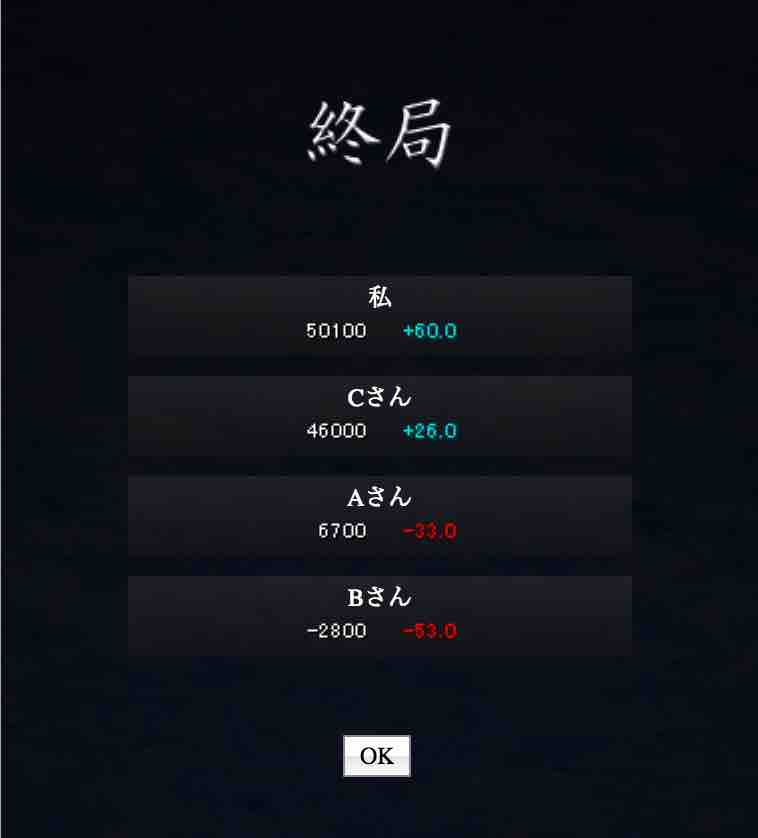
\includegraphics[width=.4\textwidth,clip]{figs/finalscore.jpg}
\end{center}
\vspace{-25pt}
\end{wrapfigure}

\bigskip

The final scores after adding {\jap uma} and {\jap oka} and scaling will be displayed along with the placements and raw scores. In the example to the right of this text, I (私 means ``me'') came in 1st, earning 50100 points (60.0 with {\jap uma} and {\jap oka}), 2nd player (C さん, which reads Mr. C) earns 46000 points (+ 26.0 with {\jap uma}), 3rd player earns 6700 points ($-33.0$ with {\jap uma}), and 4th player went bankrupt ($-2800$ points, $-53.0$ with {\jap uma}). 

\newpage
\begin{boxnote} \small
{\bf\normalsize Notes on placement}

\bigskip
It is important to keep in mind that your rank and rating on {\jap tenhou} depend solely on the placement in a game and not on how many points you earn in a game, before or after adding {\jap uma} and {\jap oka}. In other words, there is \emph{absolutely} no difference between getting 1st place with 30000 points and getting 1st place with, say, 80000 points in terms of their contributions to your rank and rating.\footnote{You might wonder why they still calculate the final scores with {\jap uma} and {\jap oka} in {\jap tenhou} if they are irrelevant; I honestly have no idea.}

\bigskip
This feature adds an interesting strategic element to the game. That is, it makes it clearer that the goal of mahjong is \emph{not} to win a hand \emph{per se} but to have a better placement at the end of a game. Winning a hand is just one of several means to securing a good placement. On occasion, you may find it beneficial to assist one of your opponents instead of trying to win a hand yourself. Intentionally dealing into an opponent's hand can sometimes be a good tactic when it serves the purpose of securing your own placement. 

\bigskip
In my impression, many European players are lacking the appreciation of this aspect of mahjong. I hope you will learn to appreciate it through playing lots of games at {\jap tenhou}.
\vspace{5pt}
\end{boxnote}

\section{Troubleshooting}

At times, you may get disconnected from the {\jap tenhou} server (possibly because of poor internet connection on your end or problems on the server).\footnote{You will notice that players sometimes get disconnected on purpose to quit playing, especially when they are losing badly.}
When a player gets disconnected from the server during a game, the game still continues. The ``auto discard draw'' will be turned on for the disconnected player, so they will be simply discarding anything they draw until they return. The player name will turn into dark red once a player is disconnected. 

%\begin{wrapfigure}{r}{60mm}
\begin{center}
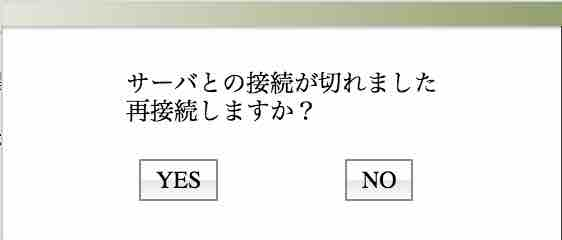
\includegraphics[width=.5\textwidth,clip]{figs/warning2.jpg}
\end{center}
%\vspace{-10pt}
%\end{wrapfigure}

When you get disconnected, you may get a warning message shown above, asking you if you would like to get connected again. Click Yes if you want to. However, a warning message does not always show up when you get disconnected. When a screen freezes during a game for more than 15 seconds, you should suspect that you are disconnected. You may want to hit the refresh button on your browser to get connected to the server again. 

\bigskip
You can create more than one accounts at {\jap tenhou}, but you will have to wait for 7 days unless your IP address changes. If you attempt to create a second account from the same IP address within 7 days, you will get an error message shown below, telling you that you cannot create a new account from your IP address in 7 days. 

\begin{center}
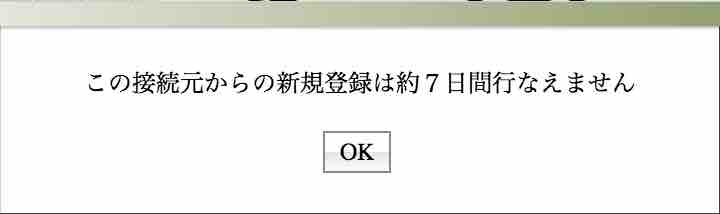
\includegraphics[width=.5\textwidth,clip]{figs/warning1.jpg}
\end{center}

\section{Rules}
Here is a summary of the rules at {\jap tenhou} games. 

\bi
\i Three red fives (one in each suit) in games with red fives.
\i No {\jap kuikae} (swap-calling). That is, you cannot discard an identical tile after {\jap pon} or {\jap chii}. You cannot discard the tile from other end of the run, either. 
\i ``Sudden death'' rule when no player has 30000 or more points after South-4 (East-4 in East-only games).
\i A game is terminated when a player goes bankrupt.
\i Automatic {\jap agariyame} rule (i.e., the game is automatically terminated if the dealer is leading after the end of South-4, even if she won a hand in South-4).
\i One-{\jap fan} minimum all the time (i.e., no two-{\jap fan} minimum even after five counters).
\i Abortive draw in the following situations
	\bi
	\i 九種九牌 (nine terminals / honors)
	\i 四家立直 (four {\jap riichi}'s)
	\i 三家和了 (three players call {\jap ron} on a discard)
	\i 四風子連打 (four players discard the same Wind)
	\i 四槓散了 (four {\jap kan} by different players)
	\ei
\i 流し満貫 ({\jap nagashi mangan}) is allowed. You can declare it even when you have called {\jap pon} / {\jap chii}. You cannot declare it if one or more of your discards has been called by others.
\i Up to two players can win on a discard. {\jap riichi} bets and counter bonus go to the player sitting closer to the player who discarded the winning tile. The dealership remains if the dealer is one of the winners.
\i The following are recognized as {\jap yakuman}: 
天和 ({\jap tenhou}; Blessing of Heaven) / 地和 ({\jap chihou}; Blessing of Earth) / 大三元 ({\jap daisangen}; Big Three Dragons) / 四暗刻 ({\jap su anko}; Four Concealed Pungs) / 四暗刻単騎 ({\jap su anko tanki}; Single-Wait Four Concealed Pungs) / 字一色 ({\jap tsuiisou}; All Honors) / 緑一色 ({\jap ryuiisou}; All Green) / 清老頭 ({\jap chinroutou}; All Terminals) / 国士無双 ({\jap kokushi muso}; Thirteen Orphans) / 国士無双13面 (Thirteen-wait Thirteen Orphans) / 大四喜 ({\jap daisushi}; Big Four Winds) / 小四喜 ({\jap shosushi}; Little Four Winds) / 四槓子 ({\jap su kantsu}; Four Kongs) / 九蓮宝燈 ({\jap churenpoutou}; Nine Gates) / 純正九蓮宝燈 ({\jap junsei churenpoutou}; Nine-wait Nine Gates).
\i {\jap Yakuman} can be combined. For example, 大三元 (Big Three Dragons) can be combined with 字一色 (All Honors), 四暗刻 (Four Concealed Pungs), and either of 四槓子 (Four Kongs), 天和 (Blessing of Heaven) or 地和 (Blessing of Earth), producing a quadruple {\jap yakuman} (128000 points). 
\i There is no double {\jap yakuman} unless different {\jap yakuman} are combined. For example, 国士無双 (Thirteen Orphans) and 国士無双13面 (Thirteen-wait Thirteen Orphans) are both single {\jap yakuman}. 
\i You cannot call {\jap pon} / {\jap chii} / {\jap kan} on the last discard in a hand. 
\i {\jap Sekinin barai}: a player who feeds the third Dragon {\jap pon} / {\jap kan} to an opponent with two melded Dragon {\jap pon} / {\jap kan} must pay the full value of the hand in case Big Three Dragons is made on a self-draw. In case another player deals into it, the two share the payment equally. The same rule applies to Big Four Winds, but not to {\jap rinshan kaihou} (After a Kong).  
\ei


\newpage

{\begin{table}[h!]\centering
\footnotesize \captionsetup{font=footnotesize}
\caption{List of {\jap yaku} names} \label{tbl:yakulist}
\begin{tabularx}{12.5cm}{l l X l}
\toprule
{\jap Yaku} & Pronunciation & EMA name & {\jap fan} (open)\\
\midrule
門前清自摸和 & {\jap (menzen-) tsumo} & Fully Concealed Hand & 1 (NA)\\
立直 & {\jap {\jap riichi}} & Riichi & 1 (NA)\\
一発 & {\jap ippatsu} & Ippatsu & 1 (NA)\\
槍槓 & {\jap chankan} & Robbing the Kong & 1\\
嶺上開花 & {\jap rinshan kaiho} & After a Kong & 1\\
海底摸月 & {\jap haitei (-moyue)} & Under the Sea & 1\\
河底撈魚 & {\jap houtei (-raoyui)} & Under the River & 1\\
自風  & {\jap jikaze} & Seat Wind & 1\\
場風  & {\jap bakaze} & Prevailing Wind & 1\\
役牌 & {\jap yakuhai} / {\jap fanpai} & Dragon Pung & 1\\
断幺九 & {\jap tanyao} & All Simples & 1\\
一盃口 & {\jap iipeiko} & Pure Double Chow & 1 (NA)\\
平和 & {\jap pinfu} & Pinfu & 1 (NA)\\
混全帯幺九& {\jap chanta} & Outside Hand & 2 (1)\\
一気通貫& {\jap ittsu} & Pure Straight & 2 (1)\\
三色同順& {\jap sanshoku (-doujun)} & Mixed Triple Chow & 2 (1)\\
三色同刻& {\jap sanshoku doukou} & Mixed Triple Pungs & 2\\
両立直 & double {\jap {\jap riichi}} & Double Riichi & 2 (NA)\\
三槓子 & {\jap san kantsu} & Three Kongs & 2\\
対々和 & {\jap toitoi} & All Pungs & 2\\
三暗刻 & {\jap san anko} & Three Concealed Pungs & 2\\
小三元 & {\jap shousangen} & Little Three Dragons & 2\\
混老頭 & {\jap honroutou} & All Terminals and Honors & 2\\
七対子 & {\jap chiitoitsu} & Seven Pairs & 2 (NA)\\
純全帯幺九 & {\jap junchan} & Terminals in All Sets & 3 (2)\\
混一色 & {\jap honitsu} & Half Flush & 3 (2)\\
二盃口 & {\jap ryanpeiko} & Twice Pure Double Chow & 3 (NA)\\
清一色 & {\jap chinitsu} & Full Flush & 6 (5)\\
流し満貫 & {\jap nagashi mangan} & All Terminals and Honors Discard & {\jap mangan}\\
ドラ & {\jap dora} & Dora & \\
赤ドラ & {\jap aka dora} & Red five & \\
裏ドラ & {\jap ura dora} & Ura dora & \\
\bottomrule
\end{tabularx}
\end{table}}
